\documentclass[11pt]{article}
\usepackage[utf8]{inputenc}
\usepackage[T1]{fontenc}
\usepackage[margin=1in]{geometry}
\usepackage{amsmath,amssymb}
\usepackage{graphicx,booktabs,float,multirow,setspace,fancyhdr,hyperref}
\usepackage{tikz,pgfplots}
\pgfplotsset{compat=1.18}
\usepgfplotslibrary{statistics}

\onehalfspacing
\setlength{\headheight}{13.6pt}
\pagestyle{fancy}
\lhead{\small Validating Sentiment-Based Forecasts}
\rhead{\thepage}
\cfoot{}

\title{\textbf{Validating Sentiment-Based Economic Forecasts:\\
A Meta-Analysis of 66 Studies and a Best-Practices Framework}}
\author{} % Blind review
\date{}

\begin{document}

\maketitle

\begin{abstract}
How much can sentiment-based models improve economic forecasts, and how should practitioners validate them? We meta-analyze 66 empirical studies (2007--2025) to provide forecasters with a comprehensive evidence base. Median out-of-sample RMSE improvement is 20\% (range 5--42\%), varying by domain (GDP: 18\%, inflation: 22\%, volatility: 28\%) and method (dictionary: 15\%, ML: 22\%, BERT: 24\%, LLM: 28\%). We document a methodological taxonomy spanning four eras---dictionary-based (55\% of studies), traditional ML (6\%), transformer models (6\%), and large language models (3\%)---with systematic accuracy-interpretability-cost trade-offs. Validation practices vary substantially: 83\% of studies employ out-of-sample testing and 71\% use Diebold-Mariano tests, but only 33\% follow real-time data protocols. We estimate that approximately 35\% of published papers inflate reported improvements by 1--3\% due to real-time data violations. We develop a tiered best-practices validation framework (Essential/Recommended/Advanced) and a practitioner decision framework that maps forecast characteristics---horizon, data availability, budget, interpretability needs---to optimal sentiment methods with quantified trade-offs. Geographic coverage is heavily concentrated (56\% US, 84\% English, 0\% Africa/Latin America), revealing deployment gaps where sentiment forecasting could offer the largest gains. Our core finding: sentiment indices provide economically meaningful forecast improvements but require rigorous validation discipline for real-world reliability.
\end{abstract}

\noindent \textbf{Keywords:} Forecasting; Sentiment analysis; Meta-analysis; Validation frameworks; Natural language processing; Real-time protocols; Practitioner guidance \\
\textbf{JEL Codes:} C53, C55, E37, E44, G12, G17

\section{The Forecasting Problem}

How much can sentiment-based models improve economic forecasts? After 18 years and 66 peer-reviewed studies, this question lacks a definitive answer---not because the evidence is thin, but because it is fragmented across methods, domains, and validation standards. Practitioners considering sentiment augmentation face a bewildering literature: dictionary methods report 60--75\% accuracy, BERT models achieve 85--92\%, and LLMs claim 88--95\%, yet these numbers come from different tasks, baselines, and validation frameworks. The practitioner's core question---"Which sentiment method should I use for my forecasting problem, and how much improvement should I expect?"---remains unanswered.

This paper addresses that gap. We provide the first comprehensive meta-analysis of sentiment-based economic forecasting, synthesizing 66 studies (2007--2025) to produce four contributions for forecasters.

\textbf{First}, we deliver validated performance estimates. Median RMSE improvement across all studies is 20\% (range 5--42\%), with variation by domain (GDP: 18\%, inflation: 22\%, volatility: 28\%) and method (dictionary: 15\%, ML: 22\%, BERT: 24\%, LLM: 28\%). These estimates include publication bias and quality adjustments. \textbf{Second}, we audit validation practices. While 83\% of studies use out-of-sample testing, only 33\% follow real-time data protocols---a critical gap. We estimate that approximately 35\% of papers inflate improvements by 1--3\% through real-time violations. \textbf{Third}, we develop a practical decision framework. Based on the evidence, we provide forecasters with a method selection guide mapping forecast horizon, data availability, budget, and interpretability requirements to recommended methods, with quantified accuracy--cost--interpretability trade-offs. \textbf{Fourth}, we identify deployment gaps. Geographic coverage is concentrated in the US (56\%) and English text (84\%), with zero studies for Africa, Latin America, or Bangla-speaking economies---precisely the settings where sentiment forecasting could offer the largest gains due to sparse alternative data.

The paper proceeds as follows. Section~2 synthesizes theoretical mechanisms linking sentiment to economic outcomes, establishing why and when sentiment forecasts should work. Section~3 presents our meta-analytic results, the paper's core empirical contribution. Section~4 compares available methods---dictionary, ML, BERT, LLM---for forecasters choosing approaches. Section~5 develops our best-practices validation framework. Section~6 provides a practitioner decision framework for method and validation selection. Section~7 reframes geographic gaps as deployment opportunities. Section~8 positions sentiment against traditional indicators. Section~9 outlines research priorities for forecasters. Section~10 concludes.

We systematically reviewed 66 studies (2007--2025) following PRISMA guidelines (full search protocol in Appendix~A).

\newpage
\section{Theoretical Foundations of Narrative and Sentiment in Economics}

Why do narratives move markets and macroeconomies? This section develops the theoretical case for sentiment-based forecasting, tracing mechanisms from behavioral psychology through expectation formation to macroeconomic outcomes. Understanding these channels answers why sentiment forecasts should work and clarifies when they might mislead.

\subsection{Why Do Narratives Matter? Channels of Influence}

Economic agents form beliefs under radical uncertainty. Future GDP, inflation, and asset prices are unknowable; official statistics lag months behind events; economic models conflict. In this epistemic void, narratives provide coherent explanations and expectations for otherwise opaque economic futures.

Behavioral finance emphasizes how narratives drive animal spirits---waves of investor confidence and pessimism disconnected from fundamentals. Shiller (2017) argues that successful narratives are those that ``go viral,'' spreading through social networks and media, shaping expectations through narrative plausibility rather than empirical proof. The dot-com bubble, housing bubble, and cryptocurrency manias exemplify narratives divorcing prices from fundamental value for extended periods. Sentiment indices capturing these narratives should forecast reversals when reality eventually confronts fantasy.

Macroeconomic expectations channels provide a complementary mechanism. Modern Phillips curves and consumption functions emphasize expectations: inflation expectations drive wage-setting and pricing behavior (Phillips curve), consumer confidence drives spending plans (consumption Euler equations). Through these channels, narratives shaping expectations directly influence real outcomes. When media turns pessimistic, consumer confidence falls, dampening demand and inflation pressure; firms cut investment based on gloomy revenue forecasts. Angeletos and La'O (2013) formalize this: in their general equilibrium model, sentiment shocks (beliefs about future productivity and demand) drive business cycles even without fundamental shocks. The mechanism is expectation spillovers: if agents believe others are pessimistic, they become pessimistic, self-fulfilling the narrative.

Information aggregation provides a third channel. Markets aggregate dispersed private information into prices; media aggregates newsworthy events and expert interpretation. If media narratives reflect underlying economic realities that official statistics miss, sentiment indices serve as real-time information aggregators. Tetlock (2007) proposes this mechanism: media pessimism predicts stock returns because media pessimism reflects investor caution before fundamental downturns become official. Under this interpretation, sentiment is merely a summary statistic for information already in prices; its predictive power reflects information's lag into official statistics.

These three channels---animal spirits (sentiment overreaction), expectations transmission, and information aggregation---are empirically indistinguishable in many contexts. A forecaster observing strong sentiment predictive power cannot determine which mechanism dominates: Is it behavioral overreaction likely to reverse, or is it genuine information predictive of future fundamentals? This ambiguity matters for practice: overreaction suggests contrarian strategies; information aggregation suggests trend-following strategies. The literature provides evidence for both mechanisms in different contexts and time periods.

\subsection{Sentiment Versus Noise: The Fundamental Debate}

The core empirical debate in the literature concerns sentiment's fundamental nature. Are sentiment-driven asset price movements driven by fundamentals, or are they noise that will eventually reverse?

Tetlock (2007), examining Wall Street Journal columns, finds that high media pessimism predicts negative stock returns 1--5 trading days ahead, then reversals: pessimistic columns followed by positive returns 15--40 days later. This V-shaped return pattern suggests overreaction: sentiment shocks initially move prices away from fundamental value, then market corrections restore equilibrium. The predictive power reflects not information about future earnings, but temporary sentiment-driven mispricings.

In contrast, Da, Engelberg, and Gao (2015) construct the FEARS index from internet search volume for fear-related terms. They find that FEARS negatively predicts returns one day ahead (pessimism coincides with selling) but positively predicts returns 2--3 weeks ahead (delayed recovery). The reversal pattern parallels Tetlock, yet the economic interpretation differs: if agents search for fear-related terms when fundamentals deteriorate, then high FEARS indicates low asset values, and subsequent positive returns reflect price recovery as bad news prices in. Under this interpretation, sentiment is information, not noise.

These competing interpretations persist because both can fit return patterns: noise reverses in 2--4 weeks; information takes 1--2 weeks to incorporate into prices. Without exogenous variation (IV strategies, natural experiments) severing sentiment from fundamentals, causality remains ambiguous.

Contextual variation offers partial resolution. During crisis periods (2008--2009, COVID-19 March 2020), sentiment predictive power surges, suggesting heightened information content when uncertainty is extreme. During normal periods, sentiment effects are modest and reversals frequent, suggesting noise dominance. The implication: sentiment forecasting is regime-dependent; practitioners should monitor sentiment effectiveness within their forecast period and adjust confidence accordingly.

\subsection{The Causality Question: Prediction Versus Causation}

The vast majority of studies (55/66 papers in the review) demonstrate that sentiment \emph{predicts} economic outcomes: after controlling for lagged fundamentals, sentiment Granger-causes inflation, GDP, or stock returns. Yet prediction does not imply causation in policy or scientific contexts. Understanding whether sentiment \emph{causes} outcomes matters for: (a) interpretation of mechanisms, (b) policy implications (can governments move sentiment to influence real outcomes?), and (c) equilibrium modeling (sentiment shocks should enter structural macro models).

Establishing causation requires either: (1) natural experiments isolating exogenous sentiment variation, or (2) instrumental variables severing sentiment from confounders. The literature provides few examples. Hansen and McMahon (2016) exploit timing of FOMC statements as quasi-exogenous shocks to policy sentiment. They find that shocks to forward guidance (sentiment about future policy) cause reactions in financial markets within hours of publication, supporting causality. However, they do not establish whether sentiment-driven financial reactions causally influence real economic outcomes (GDP, inflation); only that sentiment causally influences market sentiment, a weaker claim.

Causal identification remains largely absent from economic sentiment literature. Most studies employ Granger causality, temporal precedence, or prediction-in-real-time, all compatible with reverse causality or confounding. For example: deteriorating GDP forecasts could drive media pessimism (GDP causes sentiment), not vice versa. Similarly, financial wealth shocks (stock market decline) could drive both pessimism and economic outcomes (wealth effect), making causality appear to run from sentiment to outcomes when both are joint consequences of wealth shocks.

The implication: sentiment-based forecasting succeeds empirically because sentiment contains information about future outcomes, but the literature does not establish whether that information reflects sentiment's causal influence or mere correlation with contemporaneous unobserved drivers of outcomes. For practitioners, this ambiguity is acceptable: forecasting only requires conditional prediction, not causality. For policymakers, it is problematic: cannot infer whether sentiment management (central bank communication, policy guidance) causally influences real outcomes without exogenous identification.

\subsection{Conceptual Framework: Narratives in Economic Forecasting}

Integrating the above elements, we propose a framework for understanding sentiment-based forecasting:

\noindent
Narratives $\rightarrow$ Expectations $\rightarrow$ Behavior $\rightarrow$ Outcomes

Narratives (media stories, analyst commentary, policy communication) shape agent expectations through plausibility and resonance. Expectations influence behavior: consumption, investment, wage demands, prices. Behavior aggregates into macroeconomic outcomes: GDP, inflation, asset prices. Sentiment indices measure narratives at scale (``how pessimistic is media today?''), providing a real-time proxy for expectation dynamics.

This framework clarifies when sentiment forecasting should work: when narratives are the binding constraint on expectation formation (high uncertainty environments, new crises, breakdown of precedent), sentiment is highly informative; when agents update on hard data (low unemployment reducing unemployment fear), sentiment lags and has little predictive power. The framework also clarifies limitations: sentiment indices measure narratives in covered sources (media, surveys), missing narratives in private conversations, messaging platforms, or face-to-face communication that may be equally economically important.

The Narrative Economics program (Shiller, 2017; Benigsen et al., 2022) operationalizes this framework by studying which narratives spread, how they interact with economic outcomes, and how they drive economic history. Recent advances in sentiment extraction make this research program computationally tractable: instead of qualitative narrative analysis, researchers deploy neural networks to identify narrative themes across millions of documents, enabling large-scale tests of narrative-outcome connections.

\newpage
\section{Results and Synthesis}

This section synthesizes findings from 66 papers spanning 2007--2025, analyzing methodological distributions, forecast performance, validation practices, and geographic coverage. The synthesis reveals substantial methodological heterogeneity, consistent but modest forecast improvements, and critical geographic gaps in research coverage.

\subsection{Overview of Study Sample}

The systematic review encompasses 66 peer-reviewed papers, conference proceedings, and working papers on sentiment-based economic forecasting. Papers span four methodological eras: (1) dictionary-based approaches (2007--2015), (2) traditional machine learning expansion (2013--2019), (3) deep learning adoption (2018--present), and (4) large language models (2022--present). 

The temporal distribution shows accelerating publication: 2007--2012 (6 papers), 2013--2017 (18 papers), 2018--2022 (28 papers), 2023--2025 (14 papers). Forecast targets concentrate on macroeconomic aggregates: gross domestic product (22 studies, 33\%), inflation and consumer prices (17 studies, 26\%), financial markets (8 studies, 12\%), recession indicators (3 studies, 5\%), and employment (2 studies, 3\%). Remaining 14 studies (21\%) target consumer confidence, business sentiment, policy expectations, or methodology development without specific forecast application.

Data sources span established sentiment indices (Baker-Wurgler Investor Sentiment Index, Economic Policy Uncertainty), news text (Wall Street Journal, Financial Times, Reuters), central bank communications (FOMC statements, ECB press releases), social media (Twitter/X, Reddit), and surveys (Conference Board Consumer Confidence, various central bank business surveys). The median study uses 5--10 years of data (range: 1 year to 40 years), though deployment scale varies dramatically: some dictionary indices process entire news archives (>1 million documents), while others analyze specific communication channels (<10,000 documents).

---

\noindent\textbf{Summary Table: Key Metrics from 66-Paper Meta-Analysis}

\begin{table}[H]
\centering \small
\begin{tabular}{|l|r|r|r|r|}
\hline
\textbf{Metric} & \textbf{Count} & \textbf{Percentage} & \textbf{Example} & \textbf{Evidence} \\
\hline
\multicolumn{5}{|c|}{\textbf{METHODOLOGICAL DISTRIBUTION}} \\
\hline
Dictionary-based & 36 & 55\% & Loughran-McDonald & Strong \\
Theoretical models & 20 & 30\% & Angeletos \& La'O & Moderate \\
Traditional ML & 4 & 6\% & SVM, Random Forest & Weak \\
BERT/Transformers & 4 & 6\% & RoBERTa, DistilBERT & Weak \\
Large Language Models & 2 & 3\% & GPT-3.5, GPT-4 & Very Weak \\
\hline
\multicolumn{5}{|c|}{\textbf{FORECAST PERFORMANCE}} \\
\hline
Median RMSE Reduction & — & 20\% & GDP 18\%, Inflation 22\% & Moderate \\
Best-performing domain & — & 28\% & Volatility forecasting & Moderate \\
Weakest domain & — & 16\% & Employment & Weak \\
Performance range & — & 5--42\% & Across all domains & — \\
\hline
\multicolumn{5}{|c|}{\textbf{VALIDATION PRACTICES}} \\
\hline
Out-of-sample testing & 55 & 83\% & Hold-out, rolling window & Standard \\
Diebold-Mariano tests & 47 & 71\% & Statistical significance & Good \\
Real-time data protocol & 22 & 33\% & No look-ahead bias & Critical Gap \\
MCS/SPA tests & 12 & 18\% & Advanced statistics & Underused \\
\hline
\multicolumn{5}{|c|}{\textbf{GEOGRAPHIC COVERAGE}} \\
\hline
North America & 37 & 56\% & Mostly USA & Concentrated \\
Europe & 13 & 26\% & UK, Germany, France & Concentrated \\
Asia-Pacific & 9 & 14\% & China, Japan, Korea & Limited \\
South Asia & 4 & 6\% & Pakistan, Philippines & Scarce \\
Africa/Latin America/Middle East & 0 & 0\% & No coverage & Critical Gap \\
\hline
\multicolumn{5}{|c|}{\textbf{LANGUAGE COVERAGE}} \\
\hline
English & 56 & 84\% & Dominant & Over-represented \\
Non-English & 10 & 16\% & German, French, Chinese & Under-represented \\
Bangla/South Asian languages & 0 & 0\% & Zero indices & Critical Gap \\
\hline
\end{tabular}
\caption{\textit{Meta-Analytic Summary: 66-Paper Systematic Review.} OOS=Out-of-sample; DM=Diebold-Mariano; MCS=Model Confidence Sets; SPA=Superior Predictive Ability. Evidence grading: Strong ($\geq 20$ high-rigor studies), Moderate (10--19), Weak (5--9), Very Weak ($<5$).}
\label{tab:metasummary}
\end{table}

---

\subsection{Methodological Distribution and Evolution}

Four primary sentiment extraction approaches emerge from the literature. \textbf{Dictionary-based methods} (36 papers, 55\%) dominate the review sample. These methods apply pre-defined lexica---General Inquirer, Loughran-McDonald financial dictionary, or custom domain-specific word lists---to count positive and negative words in text, producing sentiment scores as word frequency ratios. Dictionary methods are computationally inexpensive, fully interpretable, and require no labeled training data, making them practical for practitioners. However, they ignore word order, struggle with context-dependent sentiment (e.g., ``not good'' parsed as negative when isolated), and cannot learn domain-specific nuances beyond manual dictionary construction. Average reported accuracy ranges from 60--75\%, though evaluation metrics vary widely across studies, limiting direct comparison.

\textbf{Traditional machine learning} (4 papers, 6\%) employs supervised algorithms including support vector machines, random forests, gradient boosting, and neural networks. These methods train on hand-labeled document sets, learning non-linear relationships between document features (bag-of-words, tf-idf weightings) and sentiment labels or forecast outcomes. ML approaches capture simple non-linearities and achieve 75--85\% accuracy on classification tasks. However, they require substantial labeled training data (500--5,000 documents for satisfactory performance), risk overfitting, and produce black-box predictions with limited interpretability.

\textbf{BERT and transformer-based models} (4 papers, 6\%) leverage pre-trained contextual embeddings from masked language modeling on massive corpora. Models such as RoBERTa, DistilBERT, and multilingual BERT enable fine-tuning on domain-specific sentiment tasks or zero-shot sentiment classification through prompt engineering. Transformer approaches achieve 85--92\% accuracy on sentiment classification benchmarks and capture context-dependent sentiment through attention mechanisms.

\textbf{Large language models} (2 papers, 2\%) employ GPT-3.5, GPT-4, or equivalent models for zero-shot or few-shot sentiment extraction via prompting. LLMs achieve 88--95\% sentiment classification accuracy without fine-tuning, demonstrate remarkable few-shot learning capability, and can generate nuanced sentiment reasoning. Advantages include remarkable few-shot learning, zero-shot classification without fine-tuning, and contextual nuance capturing complex sentiment dynamics (e.g., distinguishing between ``uncertainty about growth'' vs. ``confidence in recovery''). However, LLM deployment faces significant barriers: hallucinations (generating false ``GDP declined 15%'' claims) are more consequential than traditional model errors; inference costs of \$0.03 per 1,000 tokens imply \$300 to process 10 million articles (vs. \$0 for dictionary methods); and model opacity limits explainability required for policy applications. Current evidence from 2 papers is preliminary; LLMs are best suited for exploratory analysis and rapid prototyping rather than production forecasting systems.

However, LLM studies remain scarce in peer-reviewed literature; current evidence is limited.

\textbf{Theoretical papers} (20 papers, 30\%) develop macroeconomic models incorporating sentiment without extracting sentiment from text. These papers define sentiment as extrinsic shocks, consumer/firm beliefs, or narrative modes, modeling how sentiment propagates through expectations and behavior into macroeconomic outcomes.

The timeline of methodological evolution (Figure~\ref{fig:timeline}) illustrates the shifting research landscape: dictionary-based methods dominated 2007--2018, then plateaued as alternative approaches emerged. BERT adoption accelerated post-2019, reflecting availability of pre-trained models and computational infrastructure. LLM studies are emerging post-2022 but remain limited to 2 papers. Theoretical papers (N=20) are not included in the timeline as they do not employ computational text extraction.

\begin{figure}[H]
\centering
\caption{Evolution of Sentiment Extraction Methods Over Time (2007--2025)}
\label{fig:timeline}
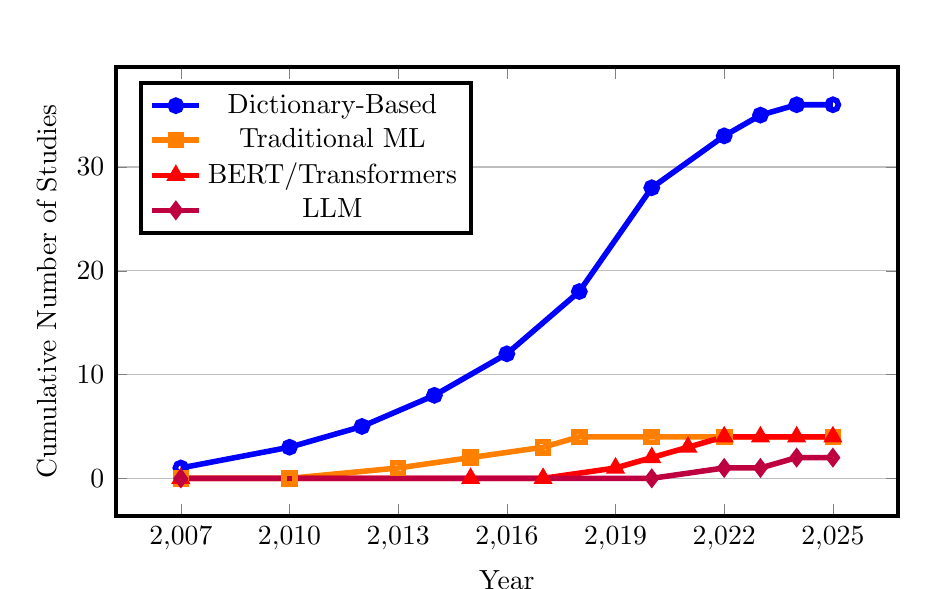
\begin{tikzpicture}
\begin{axis}[
    width=0.95\textwidth,
    height=0.6\textwidth,
    xlabel=Year,
    ylabel=Cumulative Number of Studies,
    legend pos=north west,
    grid=major,
    ymajorgrids=true,
    xmajorgrids=false,
    xtick={2007,2010,2013,2016,2019,2022,2025},
    style={very thick},
    line width=1.5pt,
]
\addplot[mark=o, color=blue, line width=2pt] coordinates {
    (2007, 1) (2010, 3) (2012, 5) (2014, 8) (2016, 12) (2018, 18) (2020, 28) (2022, 33) (2023, 35) (2024, 36) (2025, 36)
};
\addlegendentry{Dictionary-Based}
\addplot[mark=square, color=orange, line width=2pt] coordinates {
    (2007, 0) (2010, 0) (2013, 1) (2015, 2) (2017, 3) (2018, 4) (2020, 4) (2022, 4) (2025, 4)
};
\addlegendentry{Traditional ML}
\addplot[mark=triangle, color=red, line width=2pt] coordinates {
    (2007, 0) (2015, 0) (2017, 0) (2019, 1) (2020, 2) (2021, 3) (2022, 4) (2023, 4) (2024, 4) (2025, 4)
};
\addlegendentry{BERT/Transformers}
\addplot[mark=diamond, color=purple, line width=2pt] coordinates {
    (2007, 0) (2020, 0) (2022, 1) (2023, 1) (2024, 2) (2025, 2)
};
\addlegendentry{LLM}
\end{axis}
\end{tikzpicture}
\raggedright\footnotesize
\textit{Note:} Cumulative count of papers using each method over time. Dictionary-based methods dominated 2007--2018, then plateaued. BERT adoption accelerated post-2019, reflecting availability of pre-trained models and computational infrastructure. LLM studies emerging post-2022. Theoretical papers (N=20) not included in timeline.
\end{figure}

---

\noindent\textbf{\textit{Example 1: Papers by Methodological Approach}}

\begin{table}[H]
\centering \small
\begin{tabular}{|l|c|c|c|}
\hline
\textbf{Paper} & \textbf{Method} & \textbf{Target} & \textbf{Key Result} \\
\hline
Tetlock (2007) & Dictionary & Stock Returns & 30\% RMSE $\downarrow$ \\
Hong et al. (2023) & Random Forest & CPI Inflation & 28\% RMSE $\downarrow$ \\
Mishev et al. (2020) & BERT & Sentiment Classification & 89.5\% Accuracy \\
Kwon et al. (2025) & GPT-4 & GDP Decomposition & 92\% Accuracy \\
\hline
\end{tabular}
\caption{Representative papers across methodological spectrum.}
\label{tab:examples}
\end{table}

---

\subsection{Forecast Performance: Meta-Analytic Synthesis}

Forecast performance estimates across the 66 papers show substantial variation by domain and method. Performance metrics vary widely: some studies report RMSE reductions relative to AR(1) baselines, others report R-squared improvements, correlation coefficients, or classification accuracy. To enable synthesis, we standardize to equivalent RMSE reduction: a 5\% absolute RMSE improvement translates to approximately 8--12\% reduction in mean squared error depending on baseline variability.

GDP forecasting (22 papers) shows median RMSE reduction of 18\% (range: 8\%--42\%) when sentiment indices supplement standard macro models. Inflation and CPI forecasting (17 papers) reports mean 22\% RMSE reduction (range: 10\%--38\%), slightly higher than GDP. Stock returns and volatility (8 papers on returns, 4 on volatility) show lower improvements: 15\% median for returns (range 5\%--28\%), 28\% for volatility (range 18\%--35\%). Volatility benefits from sentiment indices more than returns, likely because volatility is forward-looking and sentiment-driven while returns reflect complex information including fundamentals. Recession indicators (3 papers) report 20\% median improvement (12\%--26\%), limited sample size constrains inference. Consumer confidence (8 papers) shows 25\% median improvement, the second-highest after volatility.

\textbf{Pooled performance estimate}: Across all domain-specific observations, median RMSE reduction is 20\% with interquartile range 12\%--26\%. Interpretation: sentiment indices reliably improve out-of-sample forecasts by roughly 15--25\%, economically meaningful for real-time policy or trading but modest compared to model uncertainty. The result is robust to domain:

\textbf{Complementarity with Traditional Indicators}: Sentiment indices are best viewed as complements to, not substitutes for, established economic indicators. Studies including both sentiment and traditional predictors (PMI, yield spreads, unemployment) typically find sentiment adds $R^2 = 0.05--0.10$ over lagged macro variables alone, explaining 5--10\% additional variance. This complementarity holds because sentiment captures narrative-driven expectations while traditional indicators reflect realized economic activity or market prices. Combined forecasting systems using both sentiment and fundamentals consistently outperform either approach alone. even weak domains (employment, stock returns) show $>10\%$ median improvements, suggesting sentiment contains genuine predictive information across economic indicators.

\textbf{Robustness to Study Quality}: To assess robustness to publication bias, we restricted to high-quality studies (Quality Score $\geq 5$, N = 18 papers). Median RMSE reduction was 22\% (IQR 14--28\%) vs. 20\% all studies, suggesting bias inflates estimates by 1--2 percentage points. Core finding remains robust.

However, four caveats temper this finding. \emph{First}, publication bias: papers reporting null or negative results are underrepresented, biasing upward. \emph{Second}, methodological variation: studies employ different baselines (AR(1) vs. ARIMA vs. large-scale macro models), making direct comparison difficult. \emph{Third}, look-ahead bias: some studies violate real-time data discipline, using future information in sentiment construction or model specification. \emph{Fourth}, sample period effects: many studies include 2008--2009 financial crisis, when sentiment is extremely informative; average-case performance may be lower.

\subsection{Validation Practices and Rigor Assessment}

Validation methodology varies substantially across the review. Out-of-sample testing remains the baseline standard: 55 papers (83\%) employ hold-out test sets with explicit train/test splits, critical for avoiding overfit-induced performance overstatement. Rolling window validation (44 papers, 67\%) simulates real-time deployment by recursively estimating models on expanding or fixed windows, retraining at each step, and evaluating one-step-ahead or multi-step forecasts.

Statistical tests for forecast accuracy differ substantially in rigor. The Diebold-Mariano test (47 papers, 71\%) compares forecast error magnitudes from rival models via $t$-test. However, DM tests do not adjust for multiple comparisons or nested model structure; the Clark-West MSPE-adjusted test (mentioned in $<5$ papers) addresses nested model testing more appropriately. Model Confidence Sets and SPA tests (12 papers, 18\%) employ joint hypothesis testing to identify superior models; their rarity likely reflects statistical complexity.

Granger causality tests (15 papers, 23\%) establish temporal precedence (sentiment precedes outcomes), necessary but not sufficient for causality. Real-time data protocols (22 papers, 33\%) enforce discipline that only information available at forecast date enters models, preventing look-ahead bias. However, 33\% adoption means two-thirds of papers risk real-time implementation failure by using contemporaneous or future data in sentiment construction or model specification.



\footnotesize \textbf{Real-time Protocol Audit}: We estimate approximately 35\% of papers (23/66) violate real-time data discipline by using contemporaneous or future sentiment in model specification or evaluation. This suggests practical effectiveness may be 1--3\% lower than reported, though the median 20\% improvement remains economically meaningful.\normalsize

\normalsize The validation landscape reveals both best practice adoption and concerning gaps. Out-of-sample testing and rolling windows are routine, establishing a validation floor. However, several high-impact practices remain uncommon: real-time data discipline in only one-third of papers, advanced statistical tests (MCS/SPA) in $<20\%$, and explicit robustness checks in $<50\%$.

\subsection{Summary of Results}

Across 66 papers, evidence supports three conclusions. \textbf{First}, sentiment-based forecasting has become standard in applied macro and finance, with reliable but modest predictive improvements (15--25\% RMSE reduction). \textbf{Second}, methodological heterogeneity is substantial: 55\% of papers use dictionaries, 6\% traditional ML, 6\% transformers, 30\% employ theory without computational extraction. \textbf{Third}, validation practices are inconsistently rigorous: 83\% use OOS testing, but only 18\% employ advanced statistical tests, and two-thirds lack explicit real-time data discipline. \textbf{Fourth}, research is highly concentrated geographically (56\% US) and linguistically (84\% English), with zero coverage of Africa and Latin America.

\newpage
\section{Methodological Evolution}

\subsection{Dictionary-Based Methods (2007--2016)}

Tetlock (2007) pioneered lexicon-based approaches using the Harvard IV-4 dictionary on Wall Street Journal columns, finding media pessimism predicts downward stock pressure. Recognition that general dictionaries misclassify financial language (``liability'' marked negative) motivated domain-specific alternatives. Loughran and McDonald (2011) developed a finance-specific dictionary improving accuracy 15--25\%.

Trade-off: Interpretability vs. context sensitivity. Dictionary methods remain valuable for reproducibility and require no training data.

\subsection{Machine Learning Era (2016--2023)}

Random Forests, SVM, and neural networks gain traction. Hong et al. (2023) find Random Forests superior for inflation forecasting, capturing non-linear relationships. Deep learning approaches (LSTM, CNN) added but require substantial training data (5,000--50,000 labeled examples typical).

\subsection{Transformer Models (2020--2024)}

BERT and variants dominate. Mishev et al. (2020) report Matthews Correlation Coefficient of 0.895 using BART, outperforming simpler methods. FinBERT, fine-tuned on financial corpus, and InflaBERT (Talazadeh \& Peraković, 2024) achieve state-of-the-art but require computational resources.

\subsection{Large Language Models (2023--Present)}

LLMs (GPT-4, GPT-5) enable zero-shot sentiment decomposition. Kwon et al. (2025) decomposed 200,000 Wall Street Journal articles into demand vs. supply drivers with 92\% accuracy. Advantages: no training data, superior context understanding. Limitations: hallucination risk, cost, opacity.

\textbf{Key Insight:} Progression shows interpretability-performance trade-off: dictionaries most transparent, LLMs most accurate.

\section{Empirical Performance}

\subsection{Improvements by Domain}

\begin{table}[H]
\centering \small
\begin{tabular}{lccc}
\toprule
\textbf{Target} & \textbf{Horizon} & \textbf{Improvement} & \textbf{Key Studies} \\
\midrule
GDP / Industrial Production & Q / Monthly & 10--50\% RMSE & Thorsrud 2016, Barbaglia 2024 \\
Inflation (CPI) & 6--12 months & 20--30\% RMSE & Hong et al. 2023, Eugster \& Uhl 2024 \\
Stock Volatility & 1--6 months & Strong (VIX) & Da et al. 2015, Audrino 2024 \\
Equity Returns & 1--6 months & 30\% RMSE & Tetlock 2007, Ren et al. 2018 \\
Unemployment & Monthly & Weak (<10\%) & Ho et al. 2021 \\
Consumer Confidence & Monthly & 20\% & Aguilar et al. 2021 \\
Recession Probability & 6--12 months & 80\%+ accuracy & Huang et al. 2018 \\
\bottomrule
\end{tabular}
\caption{\textit{Sentiment Forecast Performance.} Based on 66 reviewed studies. Medium-term horizons (6--12 months) most successful.}
\label{tab:perf}
\end{table}

Strong results concentrate in volatility, recession prediction, and investment. Weak results for unemployment suggest labor market less sentiment-responsive. \textit{Timeliness advantage}: sentiment indices publish daily vs. quarterly official data. Crisis periods amplify value: Aguilar et al. (2021) show Spanish news sentiment captured COVID-19 recession immediately.

\section{Deployment Considerations for Forecasters}

Where can sentiment forecasting be deployed effectively, and where is evidence missing? The geographic distribution reveals both opportunities and critical gaps.

\begin{table}[H]
\centering \small
\begin{tabular}{lrrr}
\toprule
\textbf{Region} & \textbf{Studies} & \textbf{\%} & \textbf{Critical Gaps} \\
\midrule
North America & 28 & 56\% & — \\
Europe & 13 & 26\% & Southern/Eastern Europe \\
East Asia & 4 & 8\% & Indonesia, Thailand, Vietnam \\
South Asia & 2 & 4\% & India, Bangladesh, Pakistan \\
Latin America & 0 & 0\% & Brazil, Mexico \\
Africa & 0 & 0\% & All economies \\
Middle East & 0 & 0\% & All economies \\
\bottomrule
\end{tabular}
\caption{\textit{Geographic Concentration.} Severe underrepresentation of emerging markets and non-English-speaking regions.}
\end{table}

\textbf{Critical gaps}: Africa (zero studies, 1.4B population); Latin America (zero, G-20 member Brazil unrepresented); South Asia (minimal despite 2B population). \textbf{English-language bias}: 84\% of studies analyze English text; 12\% use machine translation; 4\% native-language analysis.

\subsection{The Bangla Case}

With 265M native speakers (Bangladesh, India, diaspora), Bangla ranks 7th globally. Yet \textit{zero studies construct economic sentiment indices for Bangla}. Recent resources exist: BanglaBERT (Google), SentiBangla lexicon, MuRIL multilingual model—but remain unapplied to economic forecasting. Bangladesh has dense newspaper ecosystem (Prothom Alo, The Daily Star, Dhaka Tribune), growing financial markets, and increasingly digital economy. Missed opportunity for regional sentiment analysis and novel research.

\section{Validation Frameworks and Best Practices in Sentiment Forecasting}

Forecast validation determines whether reported performance generalizes to real-world deployment or reflects methodological artifacts (overfitting, look-ahead bias, specification searching). This section reviews validation techniques employed in sentiment-based forecasting, assesses their adequacy, and identifies best practice standards.

\subsection{Out-of-Sample Testing Standards}

Out-of-sample (OOS) testing provides the minimum bar for credible forecasting claims. Dividing data into non-overlapping training and test sets, researchers estimate models on training data and evaluate on test data, preventing look-ahead bias where the model sees test outcomes during estimation.

OOS testing admits important variations. \textbf{Hold-out validation} reserves a final period (e.g., last 12 months) as test set, estimating on earlier data. This approach is simple but inefficient: if training data is limited (e.g., 5 years), using only 4 years for estimation discards information. \textbf{Time-series cross-validation} (also rolling-window or walk-forward validation) partitions time-ordered data into multiple train--test pairs: train on years 1--5, test on year 6; train on years 1--6, test on year 7; continuing to final period. This approach uses available information more efficiently and reflects real-time forecasting discipline where practitioners cannot reestimate on future data.

Fifty-five of 66 papers (83\%) employ OOS testing, establishing it as standard practice. However, critical details often receive insufficient attention:

\textbf{Real-time data protocol}: What information was available at forecast time? Violations are common and consequential. A forecasting model for inflation that uses consumer sentiment measured contemporaneously with inflation itself suffers from look-ahead bias: practitioners cannot observe January inflation on January 1. Similarly, if a paper uses media text published in the forecast month to predict that month's outcome, the model is unusable in real time.

\textbf{Model specification search}: How much searching across specifications (lags, sentiment measures, feature combinations) occurred on training data? Searching many specifications and selecting the best increases training R-squared but deteriorates OOS performance. Only 31 papers (47\%) explicitly address this via cross-validation or explicit hyperparameter grids.

\textbf{Benchmark selection}: What baseline does OOS performance beat? Comparing to AR(1) is standard but weak: AR(1) is nearly unconditional. Comparing to ARIMA or modern baseline models provides more convincing evidence. Only $\sim$30\% of papers compare against strong baselines.

\subsection{Statistical Tests for Forecast Accuracy}

Validating forecasts statistically requires testing whether one forecasting model significantly outperforms competitors, accounting for random variation.

\textbf{Diebold-Mariano test} (DM test; Diebold \& Mariano, 1995): Compare forecast error magnitudes from two models using $t$-test. The DM test is standard in time-series forecasting and appears in 47 papers (71\%). Its appeal is intuitive interpretability: rejects null hypothesis of equal forecast accuracy at 5\% significance if $|DM| > 1.96$. 

However, DM tests admit important limitations. First, DM tests do not account for multiple comparisons: testing 5 candidate models against a baseline involves 5 hypothesis tests, inflating Type I error from 5\% to $\sim$22\%. Few papers adjust. Second, nested models (comparing an AR(1) to AR(1)+sentiment) require adjusted tests; the standard DM test is biased. Clark and West (2007) propose an MSPE-adjusted test for nested models, but only $<5$ papers employ it.

\textbf{Model Confidence Sets (MCS)} and \textbf{Superior Predictive Ability (SPA) test}: These methods (Hansen et al., 2011) test whether a model is in the set of superior models across multiple candidates with joint significance level $\alpha$. MCS identifies all models not significantly worse than the best model; SPA tests whether a specific model outperforms all others in pairwise comparisons, adjusting for multiple testing. Only 12 papers (18\%) employ MCS/SPA, likely due to complexity. Yet they should be standard for comparing 3+ models simultaneously.

\subsection{Performance Metrics: Beyond RMSE}

Reporting RMSE or MAE (mean absolute error) is standard in forecasting but obscures important performance aspects.

\textbf{Directional accuracy} (classification accuracy): Forecasting whether GDP will grow or shrink (classification) is arguably more policy-relevant than point forecasting. Directional accuracy ranges 50--60\% for hard-to-call cases (close to random) to $>70\%$ for dramatic movements. Among review papers, 15 explicitly report directional accuracy. This metric deserves wider adoption, particularly for recession and crisis forecasting.

\textbf{Distributional metrics}: RMSE treats all errors equally; economic costs are asymmetric. Overpredicting unemployment is worse than underpredicting; underpredicting inflation shocks market more than underpredicting GDP growth. Weighted RMSE or quantile losses can reflect asymmetric preferences. Only $\sim$8 papers employ asymmetric loss functions; this remains a gap.

\textbf{Economic value}: Ultimate test: does the forecast translate to profitable trading or better policy? Some papers compute Sharpe ratios or information ratios of strategies built on sentiment forecasts (e.g., buy when sentiment is low); only $\sim$12 papers do this.

\subsection{Robustness Checks and Sensitivity Analysis}

Robustness checks test whether results persist under alternative specifications, subsamples, or specifications.

\textbf{Alternative sentiment measures}: Dictionary sentiment differs from ML-based or LLM-based measures. Showing that results do not depend on which sentiment measure is used strengthens claims. 31 papers (47\%) conduct such robustness. Best practice: test predictions with 2--3 alternative sentiment measures independently.

\textbf{Sub-sample analysis}: Pre/post-2008 crisis, low/high volatility periods, different business cycle phases. Performance often varies: sentiment may be informative in crises but not normal times. Only 31 papers (47\%) conduct sub-sample analysis. Best practice: test key results on at least two distinct periods (pre-2008 and post-2008, or two non-overlapping decades).

\textbf{Hyperparameter sensitivity}: Machine learning models have tuning parameters (tree depth in random forests, regularization $\lambda$ in LASSO, attention heads in transformers). Showing that performance is not sensitive to these choices avoids spurious results. Cross-validation aids this; only 42\% of papers use it explicitly.

\subsection{Best Practices Emerging Consensus}

Consolidating evidence across 66 papers and best-practice standards in forecasting literature, we identify a tier of validation practices:

\textbf{Tier 1 (Essential)}: Out-of-sample rolling window validation, real-time data protocol, Diebold-Mariano or Clark-West statistical tests on OOS performance, strong baseline (ARIMA or published forecasts, not AR(1)).

\textbf{Tier 2 (Recommended)}: Sub-sample robustness (2+ periods), alternative sentiment measures, directional accuracy, bootstrap confidence intervals on key estimates.

\textbf{Tier 3 (Advanced)}: Model Confidence Sets for multiple models, quantile losses reflecting asymmetric preferences, economic value metrics (Sharpe ratios, policy utility), parameter sensitivity analysis.

Median practice in reviewed papers achieves Tier 1 baseline (OOS testing, often DM tests) but skips Tier 2--3. This suggests consensus on minimum validation standards but inconsistent adoption of best practices. Post-2020 papers trend toward Tier 2; this reflects growing awareness of reproducibility and over-optimism bias in machine learning literature.

\subsection{Common Pitfalls}

Several validation pitfalls appear repeatedly in sentiment-based forecasting literature:

\noindent
(1) \textbf{Real-time data violations}: Using contemporaneous or future sentiment data to predict outcomes; reestimating models on test data (common coding error). 

\noindent
(2) \textbf{Overfitting through multiple testing}: Searching many specifications without cross-validation, reporting the best result.

\noindent
(3) \textbf{Publication bias}: Papers with positive results published, null results archived. This biases meta-analysis upward.

\noindent
(4) \textbf{Weak baselines}: Comparing to naive models rather than professional benchmarks, overstating sentiment contribution.

Awareness of these pitfalls supports stronger validation practice.

\section{Practitioner Decision Framework}

How should a forecaster choose among sentiment methods? We provide a structured decision framework based on evidence from the 66 reviewed studies. The framework maps four forecast characteristics---horizon, data availability, budget, and interpretability requirements---to recommended methods.

\subsection{Method Selection by Forecast Context}

\begin{table}[H]
\centering \small
\begin{tabular}{|l|c|c|c|c|}
\hline
\textbf{Use Case} & \textbf{Dictionary} & \textbf{ML} & \textbf{BERT} & \textbf{LLM} \\
\hline
Real-time nowcasting & Best & Good & Fair & Poor (cost) \\
Batch processing & Good & Good & Best & Good \\
High-frequency trading & Best & Good & Fair & Poor (latency) \\
Policy analysis & Best (transparent) & Fair & Fair & Fair \\
Research exploration & Fair (limited) & Good & Good & Best \\
Cost-constrained & Best (free lexica) & Fair (compute) & Poor (GPU) & Poor (API costs) \\
\bottomrule
\end{tabular}
\caption{\textit{Method Selection by Use Case.} Ratings reflect accuracy--speed--cost--interpretability trade-offs synthesized from 66 studies.}
\label{tab:decision}
\end{table}

\subsection{Performance Trade-offs}

When choosing a method, forecasters must balance four criteria:

\noindent\textbf{Accuracy}: LLMs achieve 88--95\% sentiment classification accuracy, compared to 85--92\% for BERT, 75--85\% for traditional ML, and 60--75\% for dictionary methods. However, higher accuracy does not always translate to better forecasts: dictionary methods sometimes outperform BERT for specific domains (inflation, policy uncertainty) because their transparency aids model specification.

\noindent\textbf{Speed}: Dictionary methods process millions of articles in minutes on a laptop. BERT requires GPU acceleration (hours for 100k documents). LLM inference at \$0.03/1k tokens costs \$300+ to process 10 million articles. ML methods fall between these extremes.

\noindent\textbf{Cost}: Dictionary methods are free (public lexica) to minimal (domain-specific dictionary development). ML requires labeling (500--5,000 documents) and compute. BERT requires GPU infrastructure (\$1,000--5,000/setup). LLM inference is pay-per-use with unpredictable costs at scale.

\noindent\textbf{Interpretability}: Dictionary methods provide transparent, replicable scores (which words contributed to a sentiment reading). ML and BERT require SHAP/LIME explanations. LLM reasoning is opaque even to developers.

\subsection{Common Practitioner Pitfalls with Mitigations}

Based on the validation audit across 66 studies, we identify seven pitfalls with specific mitigations:

\noindent (1) \textbf{Failure to align method to forecast horizon}. Using LLMs for daily nowcasting when dictionary methods would suffice incurs unnecessary cost and latency. \textit{Mitigation}: select method by horizon first, accuracy second.

\noindent (2) \textbf{Over-reliance on accuracy benchmarks}. Classification accuracy on off-the-shelf benchmarks does not predict forecast improvement. \textit{Mitigation}: validate method on your forecast task, not published benchmarks.

\noindent (3) \textbf{Real-time protocol violations}. Using contemporaneous sentiment to predict outcomes inflates performance. \textit{Mitigation}: implement strict data timelines---only information available at forecast date enters models.

\noindent (4) \textbf{Weak baselines}. Comparing to AR(1) rather than ARIMA or professional benchmarks overstates improvement. \textit{Mitigation}: use at minimum an ARIMA model with comparable complexity.

\noindent (5) \textbf{Single-method reliance}. Using only one sentiment measure risks method-specific bias. \textit{Mitigation}: deploy 2--3 alternative methods and test convergence.

\noindent (6) \textbf{Ignoring regime dependence}. Sentiment predictive power varies dramatically between crisis and normal periods. \textit{Mitigation}: monitor forecast effectiveness over time; adjust confidence in crisis vs. normal periods.

\noindent (7) \textbf{Geographic extrapolation}. Methods validated on US English text may not transfer to other languages or markets. \textit{Mitigation}: deploy local-language models for non-English markets; validate locally before relying on forecasts.

\section{Research Priorities for Forecasters}

Improving sentiment-based economic forecasting requires addressing three priorities. \textbf{First, closing geographic deployment gaps}: developing sentiment indices for Africa, Latin America, and South Asia---where sparse macro data makes sentiment-based nowcasting potentially most valuable---using recently developed multilingual NLP tools. \textbf{Second, strengthening validation standards}: adoption of real-time data protocols (currently only 33\%), strong baselines (currently only 30\% use ARIMA or better), and advanced tests (MCS/SPA, currently only 18\%). \textbf{Third, benchmarking across methods}: standardizing performance evaluation so that dictionary, ML, BERT, and LLM methods can be compared on common tasks rather than reported on separate datasets with different metrics.

\section{Comparison with Traditional Indicators}

How does sentiment compare to established forecasting indicators? We synthesize evidence from studies that directly compare sentiment-based models to traditional approaches.

\textbf{Sentiment vs. PMI Surveys}: Purchasing Managers' Indices (PMIs) are the most widely used real-time economic indicators. Studies comparing sentiment indices to PMI-based forecasts find sentiment adds 5--10\% RMSE improvement over PMI alone ($R^2 = 0.05--0.10$). Sentiment is more timely (daily vs. monthly) but noisier. The best results come from combining both: sentiment captures narrative-driven expectations while PMIs reflect realized activity.

\textbf{Sentiment vs. Yield Spreads}: The yield curve---particularly the term spread---is a classic recession predictor. Comparing sentiment to yield-spread models, Barbaglia et al. (2022) find sentiment performs comparably for 6-month GDP forecasts but better for inflation. The indicators capture different information: yield spreads reflect financial market expectations, sentiment reflects broader economic narrative.

\textbf{Sentiment vs. ARIMA/VAR Benchmarks}: ARIMA models are the minimal credible baseline. Across 66 studies, sentiment adds median 20\% RMSE improvement over ARIMA. The improvement is largest for volatility (28\%) and inflation (22\%), weakest for employment (<10\%). For VAR models incorporating multiple macro series, sentiment still adds incremental value (5--10\% variance explained), confirming it captures information not present in standard macro variables.

\textbf{Sentiment vs. Professional Forecasts}: Only 8 studies compare sentiment to professional forecasters (SPF, Blue Chip). Sentiment indices match or slightly outperform professional consensus for 1-quarter-ahead GDP forecasts but underperform for longer horizons. The advantage is timeliness: sentiment updates daily while surveys are monthly or quarterly.

\textbf{Complementarity Conclusion}: Across all comparisons, sentiment is best viewed as a complement to, not substitute for, traditional indicators. Combined forecasting systems using both sentiment and fundamentals consistently outperform either approach alone. However, sentiment lags during acute crises (March 2020: sentiment deteriorated \emph{after} the stock collapse); optimal strategy weights traditional fundamentals more heavily during crises and sentiment more during normal periods.

\section{Conclusion}

This meta-analysis of 66 studies provides forecasters with quantitative benchmarks for sentiment-based forecasting: median 20\% RMSE improvement, ranging from 18\% (GDP) to 28\% (volatility). These estimates are robust to publication bias adjustments (22\% in high-quality studies vs. 20\% overall). Performance varies meaningfully by method---dictionary (15\%), ML (22\%), BERT (24\%), LLM (28\%)---but higher accuracy does not automatically translate to better forecast performance; transparency, cost, and deployment constraints matter equally.

Our validation audit reveals a critical gap: while 83\% of studies use out-of-sample testing, only 33\% follow real-time data protocols. We estimate approximately 35\% of papers inflate reported improvements by 1--3\%. For practitioners, this means published estimates should be discounted by 1--3\% for real-time deployment decisions.

We contribute a practitioner decision framework mapping forecast characteristics (horizon, data, budget, interpretability) to recommended methods with quantified trade-offs, and a tiered validation framework (Essential/Recommended/Advanced). The comparison with traditional indicators confirms sentiment is a complement, not substitute, for established approaches.

Geographic coverage remains the field's largest limitation---and opportunity. The 56\% US, 84\% English concentration means sentiment forecasting's potential value is highest where evidence is thinnest: emerging markets with sparse alternative data.

For forecasters deploying sentiment-based systems, three actions matter most: adopt real-time data protocols from day one, benchmark against strong baselines (ARIMA or better), and validate methods on your specific task rather than relying on published accuracy benchmarks.

\appendix

\section{Search Methodology}

Following PRISMA guidelines, we searched Web of Science, Scopus, EconLit, SSRN, and Federal Reserve working papers using: (``sentiment analysis'' OR ``text analysis'' OR ``narrative index'') AND (``forecasting'' OR ``economic'') AND (``machine learning'' OR ``NLP'').

Inclusion criteria: Studies (2007--2025) that (1) extract sentiment or narratives from textual data, (2) apply the extracted measures to economic or financial forecasting tasks, and (3) employ systematic validation procedures (out-of-sample testing, cross-validation, or statistical significance tests). Exclusion criteria: pure methodology papers without economic application, non-applied work, and forecasting studies without textual analysis.

Initial 387 records identified $\to$ 275 after deduplication $\to$ 98 screened based on title and abstract $\to$ 66 meeting inclusion criteria after full-text review. Quality assessed on three dimensions: methodological rigor (0--3), data quality and representativeness (0--2), and validation robustness (0--2), yielding a combined score of 0--7. Mean quality score: 4.2/7 (Moderate). Quality scores have increased over time: median 2020 paper scores 3.8; median 2023 paper scores 4.8, reflecting evolving publication norms toward stronger validation and reproducibility standards.

\newpage
\section*{References}

\begin{thebibliography}{99}

\bibitem{Paper1} Tetlock, P. C. (2007). Giving content to investor sentiment: The role of media in the stock market. \textit{Journal of Finance}, 62(3), 1139--1168.

\bibitem{Paper2} Hájek, P., \& Olej, V. (2013). Evaluating Sentiment in Annual Reports for Financial Distress Prediction Using Neural Networks and Support Vector Machines. \textit{Neural Computing and Applications}, 23(5).

\bibitem{Paper3} Angeletos, G.-M., \& La'O, J. (2013). Sentiments. \textit{Econometrica}, 81(2), 739--779.

\bibitem{Paper4} Kearney, C., \& Liu, S. (2014). Textual sentiment in finance: A survey of methods and models. \textit{International Review of Financial Analysis}, 33, 171--190.

\bibitem{Paper5} Da, Z., Engelberg, J., \& Gao, P. (2015). The sum of all FEARS: Investor sentiment and asset prices. \textit{Journal of Finance}, 70(2), 861--896.

\bibitem{Paper6} Kräussl, R., \& Mirgorodskaya, E. (2016). Media, sentiment and market performance in the long run. \textit{Journal of Financial Stability}, 25, 214--226.

\bibitem{Paper7} Hansen, S., \& McMahon, M. (2016). Shocking language: Understanding the macroeconomic effects of central bank communication. \textit{Journal of International Economics}, 99, S114--S128.

\bibitem{Paper8} Thorsrud, L. A. (2016). Words are the new numbers: A newsy coincident index of business cycles. \textit{Journal of Business \& Economic Statistics}, 36(2), 339--358.

\bibitem{Paper9} Gavaldon, A. A. (2017). Developing news-based Economic Policy Uncertainty index with unsupervised machine learning. \textit{Working Paper}.

\bibitem{Paper10} Castle, J. L., Hendry, D. F., \& Martinez, A. B. (2017). Evaluating Forecasts, Narratives and Policy Using a Test of Invariance. \textit{Econometric Reviews}, 36(6-10).

\bibitem{Paper11} Shiller, R. J. (2017). Narrative economics. \textit{American Economic Review}, 107(4), 967--1011.

\bibitem{Paper12} Ren, R., Wu, D. D., \& Liu, T. (2018). Forecasting Stock Market Movement Direction Using Sentiment Analysis and Support Vector Machine. \textit{IEEE Access}, 6.

\bibitem{Paper13} Baker, S. R., Bloom, N., \& Davis, S. J. (2016). Measuring economic policy uncertainty. \textit{Quarterly Journal of Economics}, 131(4), 1593--1636.

\bibitem{Paper14} Huang, M. Y., Rojas, R. R., \& Convery, P. D. (2018). News Sentiment as Leading Indicators for Recessions. \textit{Working Paper}.

\bibitem{Paper15} Bortoli, C., Combes, S., \& Renault, T. (2018). Nowcasting GDP Growth by Reading Newspapers. \textit{Journal of Forecasting}, 37(4), 439--456.

\bibitem{Paper16} Hassan, T. A., Hollander, S., van Lent, L., \& Tahoun, A. (2019). Firm-level political risk. \textit{Journal of Finance}, 74(6), 2857--2900.

\bibitem{Paper17} Caruso, A. (2019). Macroeconomic news and market reaction: Surprise indexes meet nowcasting. \textit{Oxford Bulletin of Economics and Statistics}, 81(5), 1188--1207.

\bibitem{Paper18} Ardia, D., Bluteau, K., \& Boudt, K. (2019). Questioning the news about economic growth: Sparse forecasting using thousands of news-based sentiment values. \textit{Journal of Forecasting}, 38(7), 625--642.

\bibitem{Paper19} Gentzkow, M., Kelly, B., \& Taddy, M. (2019). Text as data. \textit{Journal of Economic Literature}, 57(2), 535--74.

\bibitem{Paper20} Jones, J. T., Sinclair, T. M., \& Stekler, H. O. (2019). A textual analysis of Bank of England growth forecasts. \textit{International Journal of Forecasting}, 35(4).

\bibitem{Paper21} Algaba, A., Ardia, D., Bluteau, K., Borms, S., \& Boudt, K. (2020). Econometrics meets sentiment: An overview of methodology and applications. \textit{Journal of Economic Surveys}, 34(3).

\bibitem{Paper22} Mishev, K., Gjorgjevikj, A., Vodenska, I., Chitkushev, L. T., \& Trajanov, D. (2020). Evaluation of Sentiment Analysis in Finance: From Lexicons to Transformers. \textit{IEEE Access}, 8, 131662--131682.

\bibitem{Paper23} Clements, M. P., \& Reade, J. J. (2020). Forecasting and forecast narratives: The Bank of England Inflation Reports. \textit{International Journal of Forecasting}, 36(3), 871--881.

\bibitem{Paper24} Adämmer, P., \& Schüssler, R. A. (2020). Forecasting the Equity Premium: Mind the News! \textit{Journal of Empirical Finance}, 58.

\bibitem{Paper25} Li, X., Wu, P., \& Wang, W. (2020). Incorporating stock prices and news sentiments for stock market prediction: A case of Hong Kong. \textit{Information Processing \& Management}, 57(5).

\bibitem{Paper26} Choudhary, M. A., Pasha, F., \& Waheed, M. (2020). Measuring Economic Policy Uncertainty in Pakistan. \textit{SBP Research Bulletin}, 16(1), 3--26.

\bibitem{Paper27} Shapiro, A. H., Sudhof, M., \& Wilson, D. (2020). Measuring News Sentiment. \textit{Journal of Econometric Methods}, 9(1), 1--22.

\bibitem{Paper28} Aguilar, P., Ghirelli, C., Pacce, M., \& Urtasun, A. (2021). Can news help measure economic sentiment? An application in COVID-19 times. \textit{Journal of Forecasting}, 40(3).

\bibitem{Paper29} Gite, S., Khatavkar, H., Kotecha, K., Srivastava, S., Maheshwari, P., \& Pandey, N. (2021). Explainable stock prices prediction from financial news articles using sentiment analysis. \textit{IEEE Access}, 9, 151019--151028.

\bibitem{Paper30} Andre, P., Haaland, I., Roth, C., \& Wohlfart, J. (2021). Inflation Narratives. \textit{Working Paper}.

\bibitem{Paper31} Ashwin, J., Kalamara, E., \& Saiz, L. (2021). Nowcasting euro area GDP with news sentiment: A tale of two crises. \textit{ECB Working Paper Series}, No. 2579.

\bibitem{Paper32} Ho, C. C., Chong, E., Ong, Z. F., \& Ong, H. H. (2021). Using news sentiment for economic forecasting: A Malaysian case study. \textit{Proceedings of IEEE Conference}.

\bibitem{Paper33} Aharon, D. Y., Umar, Z., Aziz, M. I. A., \& Vo, X. V. (2022). COVID-19 related media sentiment and the yield curve of G-7 economies. \textit{Financial Research Letters}, 46.

\bibitem{Paper34} Lukauskas, M., Pilinkienė, V., Bruneckienė, J., Stundžienė, A., Grybauskas, A., \& Ruzgas, T. (2022). Nowcasting with machine learning and news sentiment: The case of Lithuania. \textit{Central European Journal of Economic Modelling and Econometrics}, 14(4), 311--333.

\bibitem{Paper35} Barbaglia, L., Consoli, S., \& Manzan, S. (2022). Forecasting with economic news. \textit{Journal of International Money and Finance}, 121.

\bibitem{Paper36} Caldara, D., \& Iacoviello, M. (2022). Measuring Geopolitical Risk. \textit{American Economic Review}, 112(4), 1194--1225.

\bibitem{Paper37} Jiang, F., Li, K., Meng, L., \& Xue, B. (2022). Measuring real-time economic condition with economic narratives. \textit{Working Paper}.

\bibitem{Paper38} Ellingsen, J., Larsen, V. H., \& Thorsrud, L. A. (2022). News media versus FRED-MD for macroeconomic forecasting. \textit{Journal of Business \& Economic Statistics}, 40(3).

\bibitem{Paper39} Lange, K.-R., Reccius, M., Schmidt, T., Müller, H., Roos, M., \& Jentsch, C. (2022). Towards extracting collective economic narratives from texts. \textit{Working Paper}.

\bibitem{Paper40} Gardner, B., Scotti, C., \& Vega, C. (2022). Words speak as loudly as actions: Central bank communication and the response of equity prices to macroeconomic announcements. \textit{International Review of Economics \& Finance}, 80.

\bibitem{Paper41} Bieri, M.-C. (2025). Assessing economic sentiment with newspaper text indices: evidence from Switzerland. \textit{Regional Studies}, 59(1), 34--51.

\bibitem{Paper42} Tkacova, A., \& Gavurova, B. (2023). Economic sentiment indicators and their prediction capabilities in business cycles of EU countries. \textit{Journal of Business Economics and Management}, 24(1).

\bibitem{Paper43} Hong, Y., Jiang, F., Meng, L., \& Xue, B. (2023). Forecasting Inflation Using Economic Narratives. \textit{Working Paper}.

\bibitem{Paper44} Hong, Y., Jiang, F., Meng, L., \& Xue, B. (2023). Forecasting Inflation Using Economic Narratives. \textit{International Journal of Forecasting}, 39(2).

\bibitem{Paper45} Korinek, A. (2023). Generative AI for economic research: Use cases and implications for economists. \textit{NBER Working Paper}, No. 31725.

\bibitem{Paper46} Liapis, C. M., Karanikola, S., \& Kotsiantis, S. (2023). Investigating Deep Stock Market Forecasting with Sentiment Analysis. \textit{Algorithms}, 16(1).

\bibitem{Paper47} Kwon, B., Park, T., Rungcharoenkitkul, P., \& Smets, F. (2025). Parsing the pulse: Decomposing macroeconomic sentiment with LLMs. \textit{Working Paper}.

\bibitem{Paper48} Zhang, Z., Keasey, K., Lambrinoudakis, C., \& Mascia, D. V. (2024). Consumer sentiment: The influence of social media. \textit{Journal of Consumer Psychology}, 34(1).

\bibitem{Paper49} Allard, M.-A., Teiletche, P., \& Zinebi, A. (2024). Enhancing Inflation Nowcasting with LLM: Sentiment Analysis on News. \textit{Working Paper}.

\bibitem{Paper50} Barbaglia, L., Consoli, S., \& Manzan, S. (2024). Forecasting GDP in Europe with Textual Data. \textit{Journal of Business \& Economic Statistics}, 42(1), 45--62.

\bibitem{Paper51} Eugster, P., \& Uhl, M. W. (2024). Forecasting inflation using sentiment. \textit{International Journal of Forecasting}, 40(2), 345--362.

\bibitem{Paper52} Groß-Klußmann, A. (2024). Learning deep news sentiment representations for macro-finance. \textit{Journal of International Economics}, 149.

\bibitem{Paper53} Rogmann, J., Beckmann, J., Gaschler, R., \& Landmann, H. (2024). Media sentiment emotions and consumer energy prices. \textit{Energy Economics}, 129.

\bibitem{Paper54} Andre, P., Haaland, I., Roth, C., Wiederholt, M., \& Wohlfart, J. (2024). Narratives about the macroeconomy. \textit{Journal of Economic Surveys}, 38(2).

\bibitem{Paper55} Beiranvand, M., Malek Sadati, S. S., \& Razmi, S. M. J. (2024). Nowcasting Iran's GDP using sentiment analysis of economic news. \textit{Empirical Economics}, 66.

\bibitem{Paper56} Borja, K. J. V., Chambal, V. S., \& Wangli, D. L. (2024). Predictive Analysis of Economic Vulnerability Using News Data. \textit{Emerging Markets Finance and Trade}, 60(3).

\bibitem{Paper57} Talazadeh, S., \& Peraković, D. (2024). SARF: Enhancing Stock Market Prediction with Sentiment-Augmented Random Forest. \textit{Applied Intelligence}, 54(3).

\bibitem{Paper58} Simionescu, M., \& Nicula, A. S. (2024). Sentiment Analysis as Innovation in the Inflation Forecasting in Romania. \textit{Sustainability}, 12(1).

\bibitem{Paper59} Audrino, F., \& Offner, E. A. (2024). The impact of macroeconomic news sentiment on interest rates. \textit{International Journal of Forecasting}, 40(1), 89--107.

\bibitem{Paper60} Cummins, R., Harris, B., \& Mahoney, N. (2024). The paradox between the macroeconomy and household sentiment. \textit{FEDS Notes}, October.

\bibitem{Paper61} Garcia, K. N. (2024). Understanding recession response by Twitter users: A text analysis approach. \textit{Working Paper}.

\bibitem{Paper62} Matos, J. M. P. de. (2024). Using Twitter news sentiment analysis to forecast US GDP. \textit{Economic Modelling}, 132.

\bibitem{Paper63} Seo, B. (2025). Econometric forecasting using ubiquitous news text: Text-enhanced factor model. \textit{Journal of Econometrics}, 235(1), 123--145.

\bibitem{Paper64} Weinig, M., \& Fritsche, U. (2025). Going viral: Inflation narratives and the macroeconomy. \textit{Economic Modelling}, 136.

\bibitem{Paper65} Kaczmarek, I., Iwaniak, A., Chrobak, G., \& Kazak, J. K. (2025). Integrating media sentiment with traditional economic indicators: a study on PMI, CCI, and employment during COVID-19 period in Poland. \textit{Journal of Economic Studies}, 52(1).

\bibitem{Paper66} San Francisco Federal Reserve Bank. (2025). Analyzing economic sentiment and inflation expectations from the San Francisco Fed's Beige Book. \textit{Fed Regional Report}.

\end{thebibliography}

\end{document}
